\documentclass[lettersize,journal]{IEEEtran}
\usepackage{amsmath,amsfonts}
\usepackage{algorithmic}
\usepackage{algorithm}
\usepackage{array}
\usepackage[caption=false,font=normalsize,labelfont=sf,textfont=sf]{subfig}
\usepackage{textcomp}
\usepackage{stfloats}
\usepackage{url}
\usepackage{verbatim}
\usepackage{graphicx}
\usepackage{cite}
\usepackage{booktabs}
\hyphenation{op-tical net-works semi-conduc-tor IEEE-Xplore}

\begin{document}

\title{Design of an 8-Bit, 250\,MS/s Binary-Weighted Current-Steering DAC in 0.18\,\textmu m CMOS}

\author{[Author 1]~and~[Author 2],~\IEEEmembership{Students,}
        \IEEEmembership{Department of Electrical Engineering, Columbia University}}

\markboth{ELEN E6316 Analog Integrated Circuit Design, Spring 2026}%
{[Author et al.]: 8-Bit 250\,MS/s DAC Design}

\maketitle

% -----------------------------------------------------------------------
\begin{abstract}
This paper presents the design of an 8-bit, 250\,MS/s digital-to-analog converter (DAC)
implemented in TSMC 0.18\,\textmu m CMOS technology with a 1.8\,V supply.
A binary-weighted current-steering architecture is adopted, consisting of eight
binary-weighted NMOS bit cells with weights 1 through 128, a transmission-gate-based
input retimer, a 100\,\textmu A NMOS-mirror bias generator, and a per-bit 6-bit
analog weight trim DAC for mismatch correction.
The differential output drives a 50\,\textOmega{}/50\,\textOmega{} resistive load from VDD,
yielding a 100\,$\Omega$ differential and 25\,$\Omega$ common-mode output impedance.
The design targets a minimum output swing of 1.5\,V peak-to-peak differential,
a spurious-free dynamic range (SFDR) exceeding 48\,dB across the Nyquist band,
and static linearity within DNL\,$<$\,$\pm$1\,LSB and INL\,$<$\,$\pm$2\,LSB.
\end{abstract}

\begin{IEEEkeywords}
Current-steering DAC, binary-weighted, 0.18\,\textmu m CMOS, SFDR, DNL, INL, analog weight tuning, input retimer
\end{IEEEkeywords}

% -----------------------------------------------------------------------
\section{Introduction}
\IEEEPARstart{H}{igh-speed} digital-to-analog converters are fundamental building
blocks in communication systems. The purpose of this project is to building
a 8-bits resokution at 250MS/s. The remainder of this paper
is organized as follows. Section ~\ref{sec:arch} describes the architecture and Section ~\ref{sec:blocks} elaborates its building
blocks. Section ~\ref{sec:sim} records the simulation results on Cadence Virtuoso. The specifications of this design presented in Table \ref{specs}.

\begin{table}[!h]
  \renewcommand{\arraystretch}{1.2}
  \caption{Design Specifications}
  \label{tab:specs}
  \centering
  \begin{tabular}{lcc}
    \toprule
    \textbf{Parameter} & \textbf{Requirement} & \textbf{Unit} \\
    \midrule
    Supply Voltage           & 1.8           & V          \\
    Sample Rate              & 250           & MS/s       \\
    Resolution               & 8             & bits       \\
    Output Type              & Differential  & --         \\
    Output Swing             & $\geq$1.5     & V$_{\text{pp,diff}}$ \\
    SFDR                     & $>$48         & dB         \\
    Diff.\ Output Resistance & 100           & $\Omega$   \\
    CM Output Resistance     & 25            & $\Omega$   \\
    Load Capacitance         & 550           & fF (each output) \\
    DNL                      & $<\pm$1       & LSB        \\
    INL                      & $<\pm$2       & LSB        \\
    Weight Tuning Range      & $\pm$10       & \%/bit     \\
    Reference Current        & 100           & \textmu A  \\
    \bottomrule
  \end{tabular}
  \label{specs}
\end{table}


% -----------------------------------------------------------------------
\section{Architecture}
\label{sec:arch}

\subsection{Binary-Weighted Current-Steering Architecture}

The DAC employs a direct binary-weighted current-steering architecture.
Eight NMOS bit cells with binary current weights ($2^k \times I_\text{unit}$, for
$k = 0, 1, \ldots, 7$) steer current to either the positive or negative output node
based on the corresponding digital input bit.
The total full-scale output current is:
%
\begin{equation}
  I_\text{FS} = I_\text{unit} \sum_{k=0}^{7} 2^k = 255\, I_\text{unit}.
  \label{eq:ifs}
\end{equation}
%
For a 1.5\,V$_{\text{pp,diff}}$ swing across the 100\,$\Omega$ differential load
(each side presents a 50\,$\Omega$ path to VDD), the required unit current is:
%
\begin{equation}
  I_\text{unit} = \frac{V_\text{swing}/2}{255 \times 50\,\Omega}
                = \frac{0.75}{12750} \approx 58.8\,\mu\text{A}.
  \label{eq:iunit}
\end{equation}

A binary-weighted topology was chosen over a segmented architecture because it
requires only 8 active cells and no thermometer decoder, minimizing digital
complexity and routing congestion.

\subsection{Analog Weight Tuning}

Device mismatch causes the actual current of each bit cell to deviate from its
ideal binary weight, degrading INL and DNL.
Each bit cell therefore incorporates an independent 6-bit trim DAC that
injects or sinks a small correction current at the internal drain node,
providing a tuning range of $\pm$10\% of the nominal cell current.
This allows per-cell calibration to recover linearity after fabrication.

\subsection{Output Network}

The differential output is terminated with two 50\,$\Omega$ resistors each
connected from VDD to the respective output node (OUTp and OUTn), plus
550\,fF capacitors from each output to ground modeling bond-pad parasitics.
This configuration yields the required 100\,$\Omega$ differential impedance
(two 50\,$\Omega$ in series for the differential mode) and 25\,$\Omega$
common-mode impedance (two 50\,$\Omega$ in parallel).
The output common-mode voltage is:
%
\begin{equation}
  V_\text{CM} = V_\text{DD} - \frac{I_\text{FS}}{2} \times 50\,\Omega.
  \label{eq:vcm}
\end{equation}

% -----------------------------------------------------------------------
\section{Building Blocks}
\label{sec:blocks}
\subsection{Top Level Design}
\begin{figure}[H]
    \centering
    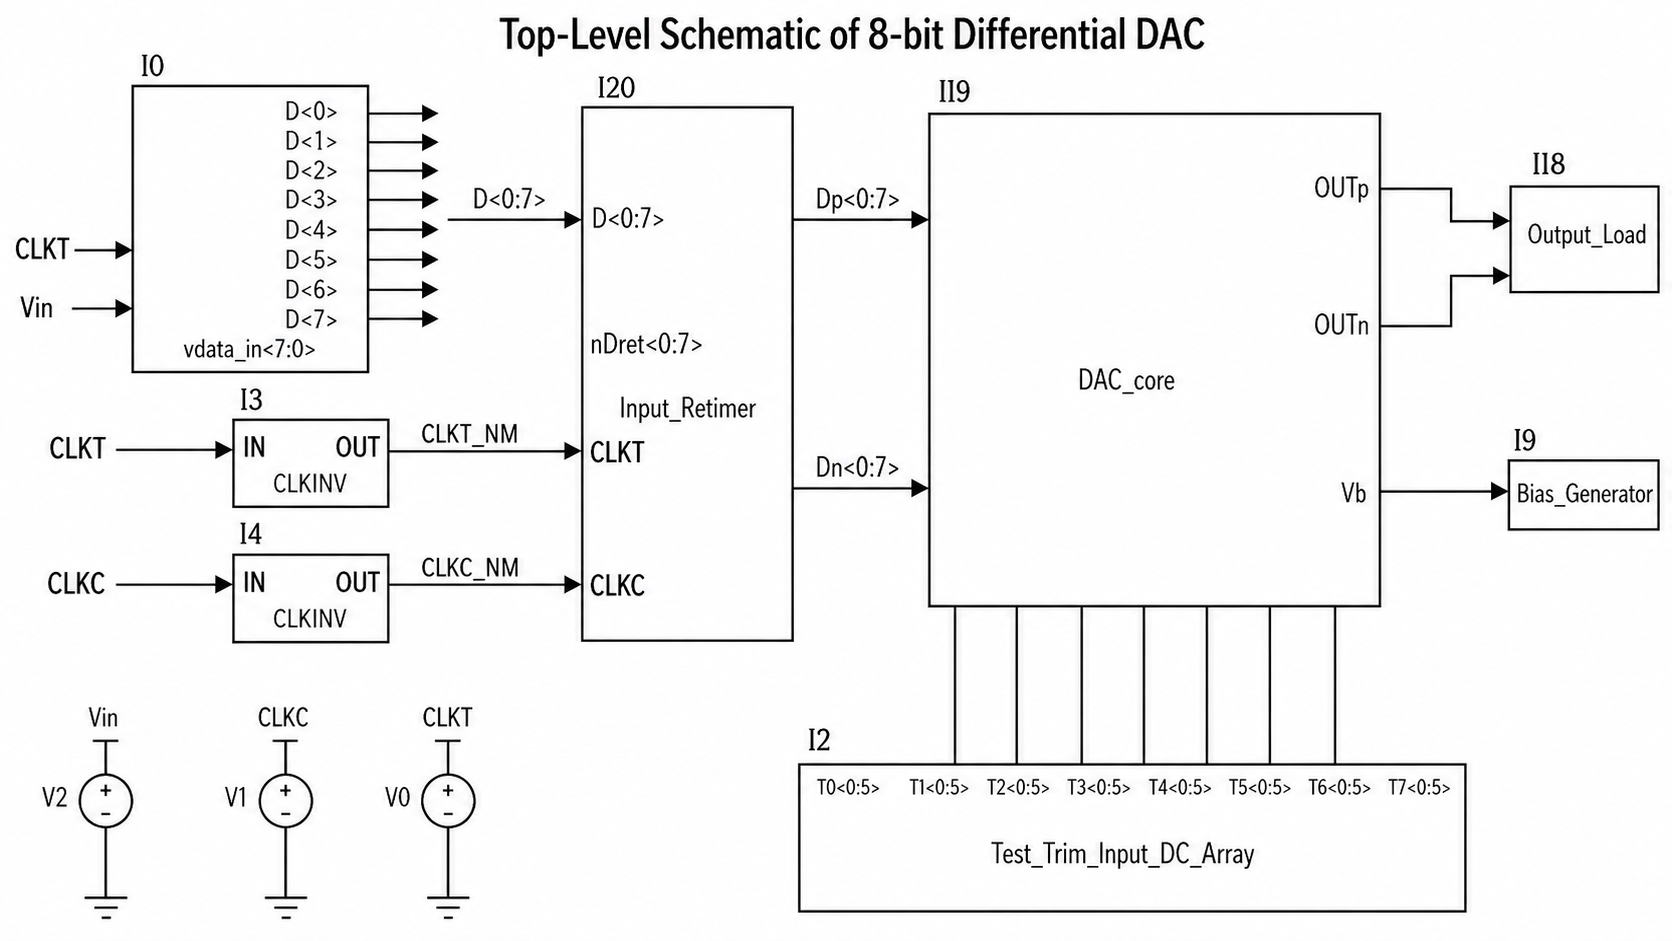
\includegraphics[width=\linewidth]{figures/top_level.png}
    \caption{Top Level Design}
\end{figure}
Blocks:
\begin{itemize}
    \item Bias Generator
    \item Input Retimeter
    \item DAC Core
    \begin{itemize}
        \item Single Bit DAC Cell
        \item Trim DAC Cell
    \end{itemize}
    \item Output Load
\end{itemize}
\subsection{Single Bit Cell of DAC Core}
The DAC core uses an 8-bit binary-weighted current-steering architecture. It contains eight bit cells with weights of 1, 2, 4, 8, 16, 32, 64, and 128, corresponding to the 8-bit input code from LSB to MSB. Each bit cell steers its weighted current to either the positive or negative output branch according to the retimed differential digital inputs $D$ and $\overline{D}$, producing a differential analog output current. A single bit cell schematics is shown in Fig \ref{fig:Bitcell}
\begin{figure}[H]
    \centering
    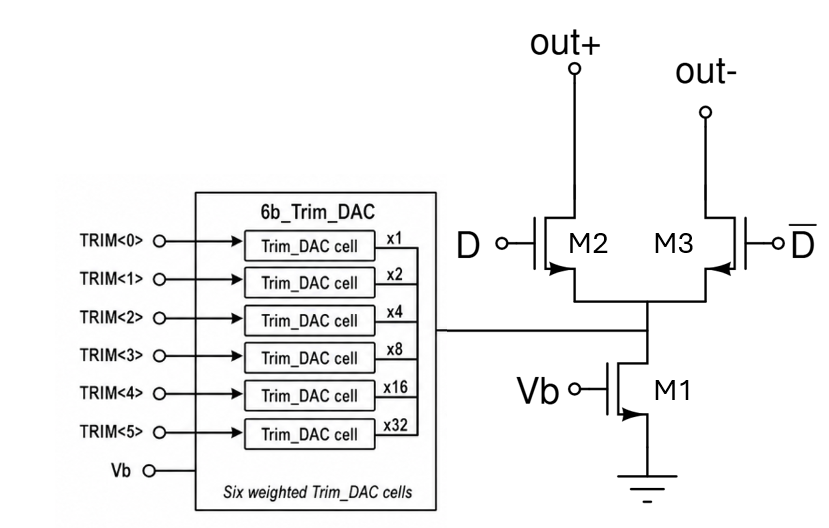
\includegraphics[width=0.9\linewidth]{figures/BitCell.png}
    \caption{Single Bit DAC Cell Tuned by a 6-bit Trim DAC}
    \label{fig:Bitcell}
\end{figure}
\begin{table}[h]
\centering
\caption{Current-Steering Switch Sizing}
\begin{tabular}{cccc}
\hline
 & W & L & Multiplier \\
\hline
M1 & 3.73 um & 1 um & weight \\
M2 & 500 nm & 180 nm & weight \\
M3 & 500 nm & 180 nm & weight \\
\hline
\end{tabular}
\end{table}
Each bit cell contains a current source M1 and input pair M2 and M3. The multiplier is defined as $m = 2^k$ is the binary multiplicity for bit $k$.
The MSB cell ($k=7$) uses $m = 128$ fingers, and the LSB cell ($k=0$) uses a
single finger.
All fingers share the same $V_b$ gate bias, so the current scales exactly with
multiplicity in the absence of mismatch.

The effective width scales with bit weight by multiplier. For example, for the MSB bit cell with weight 128, the effective width of M2 is:
\begin{equation}
    W_{eff, M2} = 500 \times 128 = 64\mu m
\end{equation}
The relative current mismatch of the unit cell is governed by threshold-voltage
and gain-factor variations:
%
\begin{equation}
  \frac{\sigma(\Delta I)}{I} =
    \sqrt{\frac{A_{VT}^2}{(V_{GS}-V_{TH})^2 \cdot WL} + \frac{A_\beta^2}{WL}},
  \label{eq:mismatch}
\end{equation}
%
with $A_{VT} = 5$\,mV$\cdot$\textmu m and $A_\beta = 0.01$\,\textmu m.
The device geometry $W \times L = 678\,\text{nm} \times 180\,\text{nm}$
was selected to satisfy the INL/DNL budget for the most sensitive bit cell.

The switch transistors M2 and M3 are scaled by the same multiplicity $m$ as the current
source so that the switch $V_\text{DS}$ and voltage headroom are consistent
across all bit cells.
\subsection{Trim DAC Cell}

Each bit cell incorporates a 6-bit Trim DAC block consisting of six
binary-weighted Single Bit Trim DAC unit cells with weights $1, 2, 4, 8, 16, 32$
times the cell's base multiplicity $m = 2^k$.

Each single bit trim DAC cell is realized by a nmos transistor accompanied by a transmission gate which is shown in Fig \ref{fig:TrimCell}
\begin{figure}[H]
    \centering
    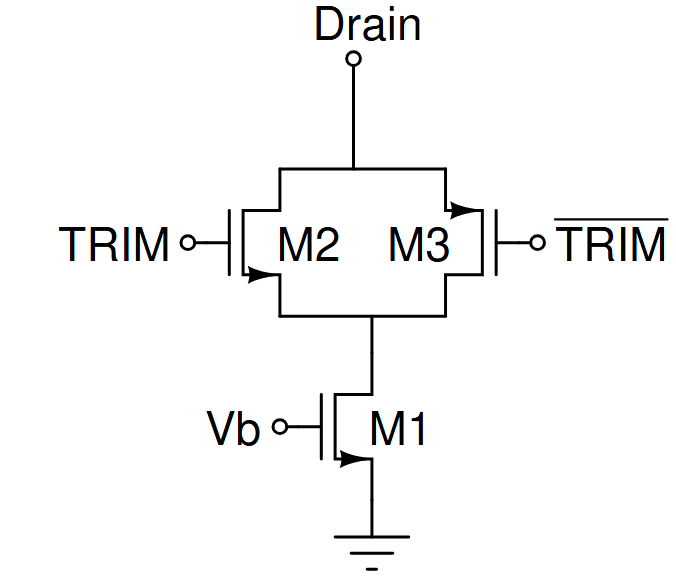
\includegraphics[width=0.5\linewidth]{figures/Trim.png}
    \caption{Single Bit Trim DAC Cell}
    \label{fig:TrimCell}
\end{figure}
\begin{table}[h]
\centering
\caption{Trim Bit Sizing}
\begin{tabular}{cccc}
\hline
 & W & L & Multiplier \\
\hline
M1 & 246 nm & 20 um & weight \\
M2 & 2 um & 180 nm & 1 \\
M3 & 2 um & 180 nm & 1 \\
\hline
\end{tabular}
\end{table}
The TRIM signal is set to 10000 by default which turns on its MSB cell. By turning off the MSB, the TRIM  drops current drew by current source in the DAC bit cell by 10\%. By turning on the rest five cells, the TRIM increases the current in DAC bit cell by 10\%. Therefore $\pm 10\%$ turning is realized.  

The completed 8-bit DAC Core is shown in Fig \ref{fig:DACCore}
\begin{figure}[H]
    \centering
    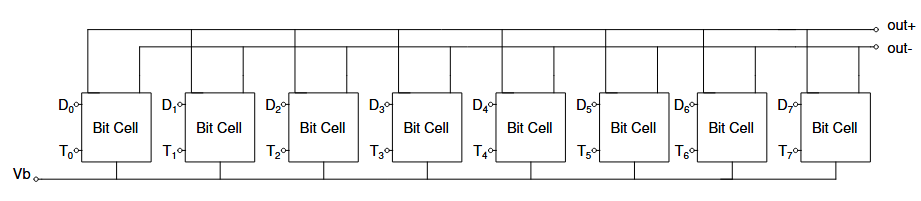
\includegraphics[width=\linewidth]{figures/DACCore.png}
    \caption{Complete 8-bit DAC Core}
    \label{fig:DACCore}
\end{figure}
\subsection{Input Retimer}

To prevent simultaneous switching glitches from arriving at the output at
different times, all 8 data bits are re-timed to the rising edge of the true
clock phase (CLK\_T) by a dedicated Input Retimer block.
Each bit passes through a Bit Retimer cell implemented static CMOS NAND-latch logic. The advantage of using NAND latch logic is to output synchronous $D_{in+}$ and $D_{in-}$ values which effectively suppress HD2 therefore increase SFDR performance. The retimer single bit cell is shown in Fig \ref{fig:RetimerCell}
\begin{figure}[H]
    \centering
    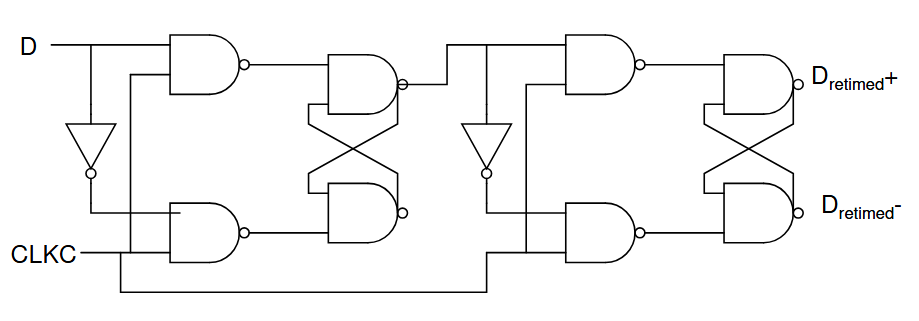
\includegraphics[width=\linewidth]{figures/RetimerCell.png}
    \caption{Single Bit Retimer Cell}
    \label{fig:RetimerCell}
\end{figure}
The NAND gate is implemented shown in Fig \ref{fig:NAND}
\begin{figure}[H]
    \centering
    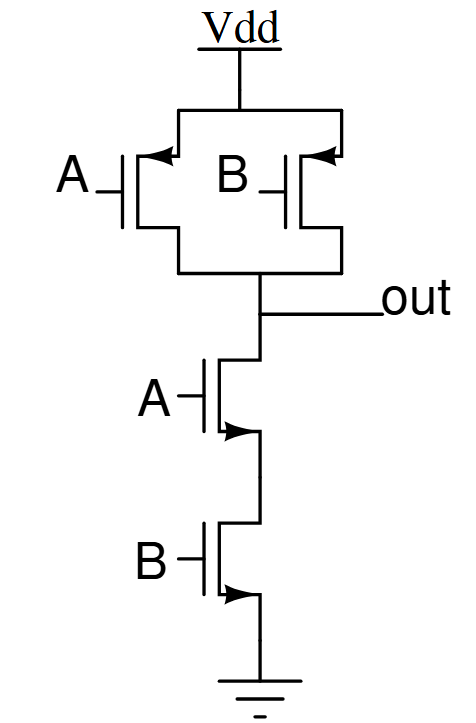
\includegraphics[width=0.4\linewidth]{figures/NAND.png}
    \caption{NAND Gate}
    \label{fig:NAND}
\end{figure}


\begin{table}[h]
\centering
\caption{Trim Bit Sizing}
\begin{tabular}{cccc}
\hline
 & W & L  \\
\hline
PMOS & 220 nm & 180 um  \\
NMOS & 220 um & 180 nm  \\
\hline
\end{tabular}
\end{table}
The completed retimer block is configured by using 8 single bit retimer cell. The completed block of retimer is shown in Fig \ref{fig:Retimer}
\begin{figure}[H]
    \centering
    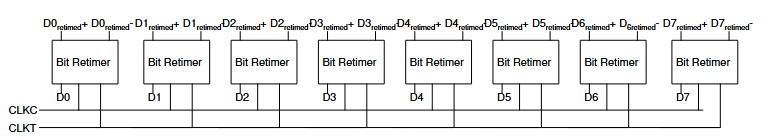
\includegraphics[width=\linewidth]{figures/Retimer.png}
    \caption{Completed Retimer Block}
    \label{fig:Retimer}
\end{figure}

This retiming ensures all bit cells switch at the same instant, suppressing
inter-bit skew and reducing dynamic nonlinearity.


\subsection{Bias Generator}

All current sources share a common gate bias $V_b$ generated by forcing
100\,\textmu A through a diode-connected NMOS transistor shown in Fig \ref{fig:Bias},
\begin{figure}[H]
    \centering
    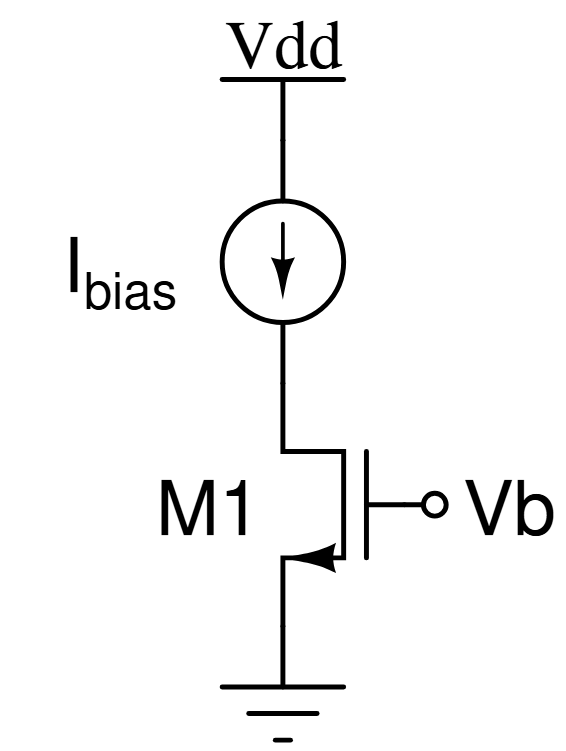
\includegraphics[width=0.3\linewidth]{figures/Bias.png}
    \caption{Bias Generator}
    \label{fig:Bias}
\end{figure}
\begin{table}[h]
\centering
\caption{Bias Parameter}
\begin{tabular}{cc}
\hline
 $I_{bias}$ & 100\,\textmu A \\
 Vdd & 1.8 V \\
 W  & 220 nm \\
 L  & 180 nm \\
 Multiplier & 4 \\
\hline
\end{tabular}
\end{table}
%
\begin{equation}
  M_\text{1}: \quad W/L = 4 \times \frac{220\,\text{nm}}{180\,\text{nm}}.
  \label{eq:biasref}
\end{equation}
%
$V_b$ is distributed to every bit cell, ensuring all currents track each other
over process and temperature variations.





% -----------------------------------------------------------------------
\section{DAC Design and Simulation Results}
\label{sec:sim}

\subsection{Simulation Setup}

Dynamic performance is evaluated using a coherent sinusoidal stimulus.
An ideal 8-bit ADC converts an analog sine wave at frequency $f_\text{in} = f_s \cdot J/M$
(with $J$ and $M$ chosen to be coprime integers) into the 8-bit digital word
fed to the DAC.
A Hanning window is applied before the FFT to suppress spectral leakage.
The simulation length is set to exactly $M$ clock cycles to ensure coherent
sampling and avoid deterministic quantization spurs.
All simulations are performed at $T = 27^\circ$C across TT, SS, and FF
process corners.

\subsection{Static Performance}

% [PLACEHOLDER: Insert INL vs. code and DNL vs. code plots.
%  Report peak INL and peak DNL values for all three corners.
%  Show current cell output current sweep demonstrating ±10% trim range
%  when the 6-bit trim code is swept from 0 to 63.]

\subsection{Dynamic Performance}

% [PLACEHOLDER: Insert FFT spectra at low input frequency (e.g., ~1 MHz)
%  and near-Nyquist (e.g., ~120 MHz). Annotate fundamental, HD2, HD3, and
%  worst-case spur. Report SFDR and SNDR at each frequency.
%  Insert SFDR vs. fin sweep plot from 0 to 125 MHz.]

\subsection{Performance Summary}

Table~\ref{tab:perf} summarizes the simulated DAC performance.

\begin{table}[!h]
  \renewcommand{\arraystretch}{1.2}
  \caption{Performance Summary (TT Corner, 27$^\circ$C)}
  \label{tab:perf}
  \centering
  \begin{tabular}{lcc}
    \toprule
    \textbf{Parameter} & \textbf{Value} & \textbf{Unit} \\
    \midrule
    DNL (peak)                           & -- & LSB \\
    INL (peak)                           & -- & LSB \\
    SFDR @ low $f_\text{in}$             & -- & dB  \\
    SFDR @ high $f_\text{in}$            & -- & dB  \\
    SNDR @ low $f_\text{in}$             & -- & dB  \\
    SNDR @ high $f_\text{in}$            & -- & dB  \\
    \midrule
    Power — Current Sources              & -- & mW  \\
    Power — Switches \& Retimer          & -- & mW  \\
    Power — Bias Generator               & -- & mW  \\
    Power — Trim DACs                    & -- & mW  \\
    \textbf{Total Power}                 & -- & mW  \\
    \bottomrule
  \end{tabular}
\end{table}

\subsection{SFDR Limiting Factors}

% [PLACEHOLDER: Identify the dominant SFDR/SNDR bottleneck (e.g., MSB current-source
%  mismatch causing HD2/HD3, switch charge injection creating spurs near fs/2,
%  or retimer skew). Support with simulation evidence such as disabling trim
%  correction or sweeping clock jitter.]

% -----------------------------------------------------------------------
\section{Conclusion}
\label{sec:conc}

% [PLACEHOLDER: Summarize achieved performance metrics, compare against the
%  specification table, and comment on which design choice most impacted
%  the SFDR/linearity tradeoff.]

% -----------------------------------------------------------------------
\end{document}
